\documentclass{article}\usepackage[]{graphicx}\usepackage[]{color}
%% maxwidth is the original width if it is less than linewidth
%% otherwise use linewidth (to make sure the graphics do not exceed the margin)
\makeatletter
\def\maxwidth{ %
  \ifdim\Gin@nat@width>\linewidth
    \linewidth
  \else
    \Gin@nat@width
  \fi
}
\makeatother

\definecolor{fgcolor}{rgb}{0.345, 0.345, 0.345}
\newcommand{\hlnum}[1]{\textcolor[rgb]{0.686,0.059,0.569}{#1}}%
\newcommand{\hlstr}[1]{\textcolor[rgb]{0.192,0.494,0.8}{#1}}%
\newcommand{\hlcom}[1]{\textcolor[rgb]{0.678,0.584,0.686}{\textit{#1}}}%
\newcommand{\hlopt}[1]{\textcolor[rgb]{0,0,0}{#1}}%
\newcommand{\hlstd}[1]{\textcolor[rgb]{0.345,0.345,0.345}{#1}}%
\newcommand{\hlkwa}[1]{\textcolor[rgb]{0.161,0.373,0.58}{\textbf{#1}}}%
\newcommand{\hlkwb}[1]{\textcolor[rgb]{0.69,0.353,0.396}{#1}}%
\newcommand{\hlkwc}[1]{\textcolor[rgb]{0.333,0.667,0.333}{#1}}%
\newcommand{\hlkwd}[1]{\textcolor[rgb]{0.737,0.353,0.396}{\textbf{#1}}}%
\let\hlipl\hlkwb

\usepackage{framed}
\makeatletter
\newenvironment{kframe}{%
 \def\at@end@of@kframe{}%
 \ifinner\ifhmode%
  \def\at@end@of@kframe{\end{minipage}}%
  \begin{minipage}{\columnwidth}%
 \fi\fi%
 \def\FrameCommand##1{\hskip\@totalleftmargin \hskip-\fboxsep
 \colorbox{shadecolor}{##1}\hskip-\fboxsep
     % There is no \\@totalrightmargin, so:
     \hskip-\linewidth \hskip-\@totalleftmargin \hskip\columnwidth}%
 \MakeFramed {\advance\hsize-\width
   \@totalleftmargin\z@ \linewidth\hsize
   \@setminipage}}%
 {\par\unskip\endMakeFramed%
 \at@end@of@kframe}
\makeatother

\definecolor{shadecolor}{rgb}{.97, .97, .97}
\definecolor{messagecolor}{rgb}{0, 0, 0}
\definecolor{warningcolor}{rgb}{1, 0, 1}
\definecolor{errorcolor}{rgb}{1, 0, 0}
\newenvironment{knitrout}{}{} % an empty environment to be redefined in TeX

\usepackage{alltt}

\usepackage{fancyhdr} % Required for custom headers
\usepackage{lastpage} % Required to determine the last page for the footer
\usepackage{extramarks} % Required for headers and footers
\usepackage{graphicx} % Required to insert images
\usepackage{hyperref}
\usepackage{amsmath} %for binomial pdf
\usepackage{parskip} % so that there's space bw paragraphs
\usepackage{float}
\usepackage{amsfonts}
\usepackage{hanging}
\usepackage{undertilde}
\usepackage{amssymb}
\usepackage{graphicx} %include images


% Margins
\topmargin=-0.45in
\evensidemargin=0in
\oddsidemargin=0in
\textwidth=6.5in
\textheight=9.0in
\headsep=0.25in 

\linespread{1.1} % Line spacing

% Set up the header and footer
\pagestyle{fancy}
\lhead{Seminar} % Top left header
\chead{LOD} % Top center header
\rhead{Pea Lodging} % Top right header
\lfoot{11/18/2016} % Bottom left footer
\cfoot{} % Bottom center footer
\rfoot{Page\ \thepage\ of\ \pageref{LastPage}} % Bottom right footer
\renewcommand\headrulewidth{0.4pt} % Size of the header rule
\renewcommand\footrulewidth{0.4pt} % Size of the footer rule

\setlength\parindent{0pt} % Removes all indentation from paragraphs
\setlength\parskip{0.5cm}
\restylefloat{table}

%----------------------------------------------------------------------------------------
%	DOCUMENT STRUCTURE COMMANDS
%	Skip this unless you know what you're doing
%----------------------------------------------------------------------------------------

% Header and footer for when a page split occurs within a problem environment
\newcommand{\enterProblemHeader}[1]{
\nobreak\extramarks{#1}{#1 continued on next page\ldots}\nobreak
\nobreak\extramarks{#1 (continued)}{#1 continued on next page\ldots}\nobreak
}

% Header and footer for when a page split occurs between problem environments
\newcommand{\exitProblemHeader}[1]{
\nobreak\extramarks{#1 (continued)}{#1 continued on next page\ldots}\nobreak
\nobreak\extramarks{#1}{}\nobreak
}


%----------------------------------------------------------------------------------------%
\IfFileExists{upquote.sty}{\usepackage{upquote}}{}
\begin{document}

\section{Setting Significance Threshold}

\subsection{LOD}
A loci is the position of a gene on a chromosome. Multiple testing problems occur often in QTL analysis as we do number phenotypes $\times$ number loci tests. Consider one phenotype, pea lodging and the 5199 loci in Jamin's study. We could set an adjusted pea-value. An alternative method Jamin would like is calculating a genome wide adjusted LOD score at each QTL and determining significance based on that threshold.

LOD is the $log_{10}$ liklihood ratio comparing the null that there is not a QTL to the alternative, that there is.

$H_{o}: y_{i} \sim N(\mu, \sigma^2)$ i.e. there is no genetic dependency between the phenotype and the genotype

- use MLEs for parameter estimates $\mu = \bar{y}; \sigma^2 = RSS_{o}/n$

$H_{a}: y_{i}|g_{i} \sim N(\mu_{g_{i}}, \sigma^2)$

- $g_{i}$ = genotype of individual i at the marker (loci); each genotype (AA,AB?) group has a different mean; $\sigma^2$ = pooled RSS = $RSS_{1}$; again the MLEs. 

LOD = $\frac{n}{2} \times log_{10}(\frac{RSS_{o}}{RSS_{1}})$

LOD is related to the F statistic.

LOD = $\frac{n}{2} \times [F({\frac{df}{n-df-1} + 1)]$ and similar to the F statistic, large LOD values are associated with strong evidence for the alternative, that there is a relationship to the genetic loci and the phenotype.

Note that if genetic information is missing, that plant cannot be included. (Section 4.1)

\subsection{Genome-wide maximum LOD}

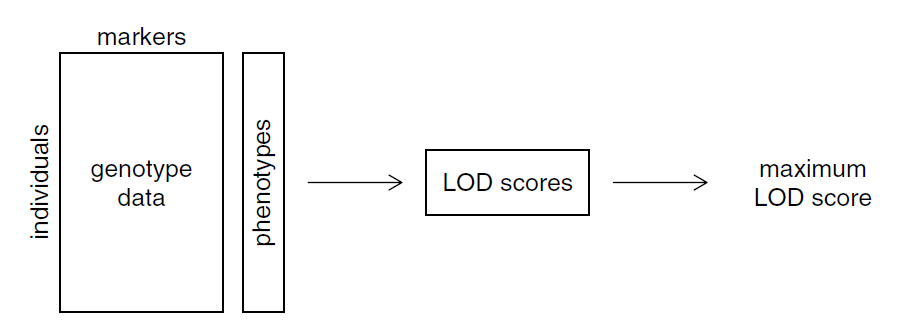
\includegraphics[scale = 0.5]{lod_pic}

Steps:
\begin{enumerate}
\item Permute the phenotypic data
\item Reassign it to the genetic data
\item Calculate LOD for each loci
\item Save the maximum LOD
\item Repeat many times -- Note there, is a calculation for the number of times to repeat
\end{enumerate}

Use the 95\%th percentile of the maximum LOD distribution as the genome wide significance threshold. It is also possible to calculate the corresponding pvalues.

Items needed:
\begin{itemize}
\item {\bf Backcross}/Intercross
\item Size of genome (in cM)
\item Number of individuals
\item Number of typed markers
\item Pattern of missing genotypic data
\item Phenotypic distribution
\end{itemize}

\section{Considerations}

\begin{itemize}
\item Section 4.7 -- ${qtl}$ does not (yet) have capabilities to do a joint analysis of multiple phenotypes, which Jamin has.

A joint analysis would increase power because we aren't conducting number phenotypes $\times$ number genetic markers tests separately. It can also allow for testing of plieotrophy (vs. tight linkage) which is whether a single QTL affects multiple phenotypes. 

\item Did he use selective genotyping?

\item The number of permutatons to run. Base this on the desired width of the pvalue CI. \url{http://www.rqtl.org/faq/}
\end{itemize}

{\bf look at notes from last time -- what is cM}

\section{References}
Information as well as the graphic was taken from:

Broman and Sen. 2009. {\it A guide to QTL mapping with R/QTL}.

\end{document}
